% In this file you should put the actual content of the blueprint.
% It will be used both by the web and the print version.

\chapter{Introduction}

This blueprint accompanies a Lean~4 formalization of Kepler's three laws of planetary motion.
It follows the proof strategy of Guillemin and Sternberg in
\href{https://bookstore.ams.org/COLL/42}{\emph{Variations on a Theme by Kepler}}.

\medskip
\noindent\textbf{The physical setup.}
We study a particle of mass $m$ moving in $\R^3$ under the gravitational attraction of a fixed body at the origin.
Its position is $q \in \R^3$ and its momentum is $p \in \R^3$.
The Hamiltonian is
\[
  H(q,p) = \frac{\|p\|^2}{2m} - \frac{\mu}{\|q\|},
\]
where $\mu > 0$ is the gravitational parameter.
The kinetic energy is $\|p\|^2/(2m)$ and the potential energy is $-\mu/\|q\|$.
We only consider \emph{non-collision} trajectories, meaning $\|q(t)\| \neq 0$ for all $t$.

\medskip
\noindent\textbf{What negative energy means.}
The condition $H < 0$ says that the total energy is negative.
The motion is then bounded.
For the inverse-square law, this is exactly the case of ellipses.
If one fixes a specific value $h < 0$, then the equation $H = h$ cuts out a five-dimensional level set inside the six-dimensional phase space.
In Lean we also keep the non-collision condition $r \neq 0$ as part of this fixed-energy surface.
This level set is often called an \emph{energy shell}.
We will usually say \emph{fixed-energy surface}.
It is just the set of phase points with that one fixed energy.

\medskip
\noindent\textbf{What we prove.}
For every non-collision trajectory with negative energy and nonzero angular momentum, we prove:

\begin{enumerate}
  \item \textbf{First law.}
    The orbit lies in a fixed plane and is an ellipse with the origin at one focus.
  \item \textbf{Second law.}
    The line from the origin to the planet sweeps area at a constant rate:
    \[
      \frac{d\mathcal{A}}{dt} = \frac{\|L\|}{2m},
    \]
    where $L = q \times p$ is the angular momentum vector.
    Equal areas are swept in equal times.
  \item \textbf{Third law.}
    If $T$ is the orbital period and $a$ is the semi-major axis, then
    \[
      T^2 = \frac{4\pi^2 m}{\mu}\,a^3.
    \]
\end{enumerate}

\medskip
\noindent\textbf{The two key conserved vectors.}
Two vector quantities stay constant along every Kepler trajectory.
The first is the angular momentum
\[
  L = q \times p.
\]
Because $L$ is perpendicular to both $q$ and $p$, its constancy immediately forces the motion to stay in one fixed plane.

The second is the Laplace--Runge--Lenz vector
\[
  A = p \times L - \frac{m\mu}{\|q\|}q.
\]
It points along the major axis of the orbit toward perihelion.
Its length records the eccentricity.
Thus $L$ determines the orbital plane and $A$ determines the ellipse in that plane.

\medskip
\noindent\textbf{Proof sketch.}
First, conservation of $L$ gives a fixed plane, so the motion is two-dimensional.
Next, the identity
\[
  A \cdot q = \|L\|^2 - m\mu r
  \qquad (r = \|q\|)
\]
turns the constancy of $A$ into the polar equation
\[
  r = \frac{\ell}{1 + e\cos\theta},
\]
which is the equation of a conic with focus at the origin.
The negative-energy condition then implies $0 \le e < 1$, so the conic is an ellipse.
That proves Kepler's first law.

Kepler's second law comes from the same conserved angular momentum:
\[
  \frac{d\mathcal A}{dt} = \frac{\|L\|}{2m}.
\]
So the areal velocity is constant.
Finally, one full period sweeps exactly the area $\pi ab$ of the ellipse, and comparing that area with the constant areal velocity gives
\[
  T^2 = \frac{4\pi^2 m}{\mu}a^3.
\]
That is Kepler's third law.

\medskip
\noindent\textbf{Momentum maps and comoment maps.}
Let $\mathfrak{g}$ be a Lie algebra acting on a phase space $M$.
A momentum map is a map
\[
  \mu \colon M \longrightarrow \mathfrak{g}^*.
\]
The corresponding comoment map is the scalar-valued map
\[
  \tilde\mu \colon \mathfrak{g} \longrightarrow C^\infty(M)
\]
given by
\[
  \tilde\mu(\xi)(x) = \langle \mu(x), \xi \rangle.
\]
The defining relation is
\[
  \bigl\{\tilde\mu(u),\,\tilde\mu(v)\bigr\} = \tilde\mu\bigl([u,v]\bigr)
  \qquad \text{for all } u, v \in \mathfrak{g}.
\]
So each $u \in \mathfrak{g}$ gives a Hamiltonian function $\tilde\mu(u)$.
Its Poisson brackets match the Lie bracket in $\mathfrak{g}$.
Lean uses this scalar-valued form.

We identify $\mathfrak{so}(3) \cong \R^3$ with bracket $[u,v] = u \times v$.
For any $u \in \R^3$, the function $L_u := u \cdot L = u \cdot (q \times p)$ is conserved.
The map $u \mapsto L_u$ is an $\mathfrak{so}(3)$-comoment: it satisfies
$\{L_u, L_v\} = L_{u \times v}$,
which is exactly the comoment condition.

\medskip
\noindent\textbf{The fixed negative-energy surface and the hidden $\mathfrak{so}(4)$ symmetry.}
The bracket identities for $L$ and $A$ depend on the energy:
\[
  \{A_u, A_v\} = -2mH\,L_{u \times v}.
\]
So the sign of $H$ matters.
When $H > 0$ one gets a different symmetry algebra.
When $H = 0$ one gets a limiting case.
For Kepler's laws for bounded orbits, the relevant case is $H < 0$.

Fix $h < 0$ and restrict attention to the fixed-energy surface $H = h$.
Because $h$ is now a fixed negative number, the quantity $-2mh$ is positive and we may rescale $A$ by the real factor $\sqrt{-2mh}$.
Define
\[
  K = \frac{A}{\sqrt{-2mh}}.
\]
This rescaling removes the factor $-2mH$ from the bracket once we are on the level set $H = h$.

On the fixed-energy surface one gets
\[
  \{K_u, K_v\} = L_{u \times v}, \qquad \{L_u, K_v\} = K_{u \times v}.
\]
The six observables $L_u$ and $K_u$ therefore satisfy the bracket relations of $\mathfrak{so}(4)$.
The map $(u, v) \mapsto L_u + K_v$ is an $\mathfrak{so}(4)$-comoment on that fixed-energy surface.
Here \emph{hidden symmetry} means an extra conserved quantity that does not come from the standard action of spatial rotations.
Without this extra conserved quantity, central-force orbits usually precess and do not close.

\medskip
\noindent\textbf{Proof in Lean.}
\begin{enumerate}
  \item Verify the equations of motion: $\dot q = p/m$ and $\dot p = -\mu q/\|q\|^3$.
  \item Prove that $L$, $A$, and $H$ are constant along every solution.
  \item Establish algebraic identities connecting $L$, $A$, and $H$, in particular $\|A\|^2 = (m\mu)^2 + 2mH\|L\|^2$.
  \item Set up the Poisson bracket and show $u \mapsto L_u$ is an $\mathfrak{so}(3)$-comoment.
  \item Prove $\{A_u, A_v\} = -2mH\,L_{u \times v}$ and then, on the fixed-energy surface $H = h < 0$, rescale to the hidden $\mathfrak{so}(4)$ symmetry.
  \item Use $L$ to get a fixed orbital plane and use $A \cdot q = \|L\|^2 - m\mu r$ to derive $r = \ell/(1 + e\cos\theta)$.
  \item Use the negative-energy identity for $\|A\|^2$ to prove $0 \le e < 1$, so the conic is an ellipse with the origin at a focus.
  \item Use the constant areal velocity to prove the second law.
  \item Combine the areal velocity with the ellipse area $\pi ab$ to obtain the period law.
\end{enumerate}

\medskip
\noindent\textbf{Geometry.}
The orbit lies in the plane perpendicular to $L$.
Inside that plane, $A$ points toward perihelion.
The origin is a focus of the ellipse.
The major axis has length $2a$.

\medskip
\noindent\textbf{Ellipse terminology.}
The major axis is the longest line through the center of the ellipse.
The minor axis is the shortest line through the center and perpendicular to the major axis.
The semi-major axis is half of the major axis.
The semi-minor axis is half of the minor axis.
If $F$ is a focus, then the latus rectum is the chord through $F$ perpendicular to the major axis.
Its half-length is the semi-latus rectum $\ell$.
For an ellipse one has $\ell = b^2/a$.

\begin{figure}[h]
\centering
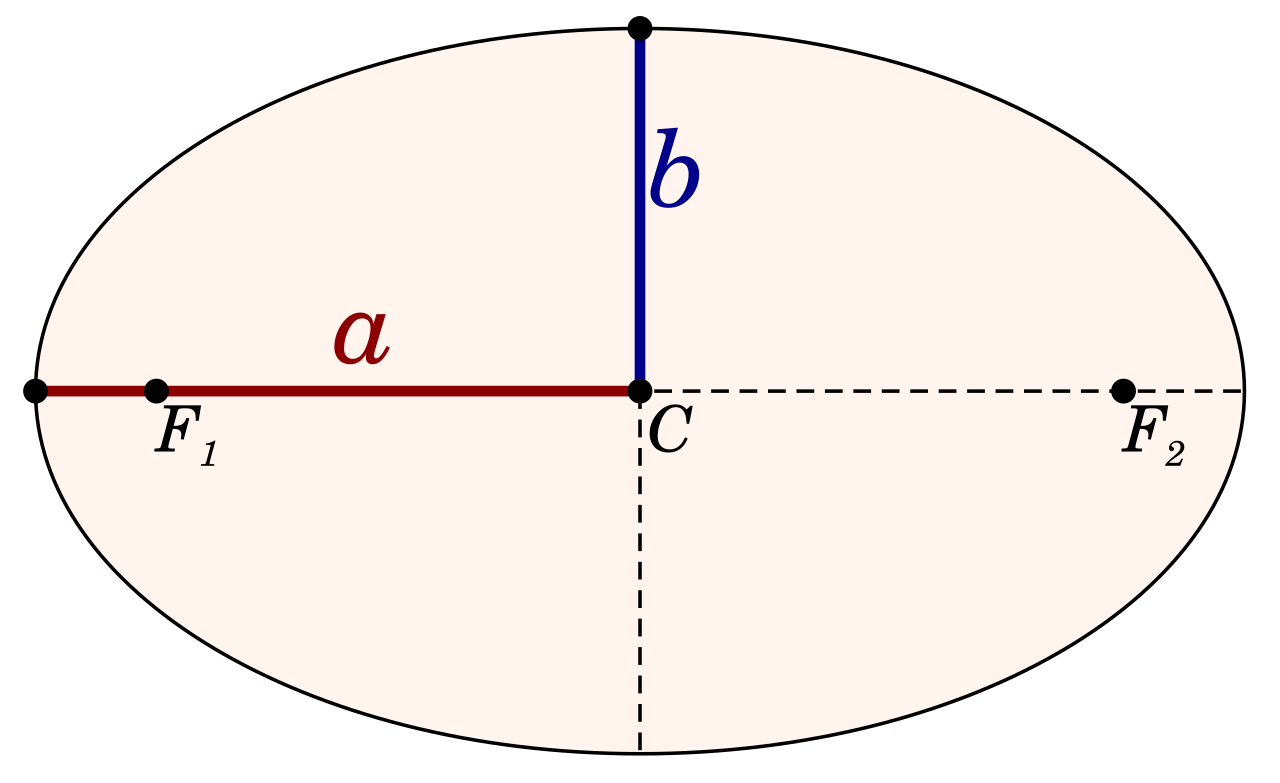
\includegraphics[width=7cm]{figures/ellipse-axes.png}
\caption{Basic ellipse axis terminology. Source: Wikimedia Commons, \href{https://commons.wikimedia.org/wiki/File:Ellipse_semi-major_and_minor_axes.svg}{``Ellipse semi-major and minor axes.svg''} by M. W. Toews. CC0 1.0.}
\end{figure}

\medskip
\noindent\textbf{Note on the Lean formalization.}
The source text works on $T^*(\R^3 \setminus \{0\})$.
The Lean development instead uses the ambient space $\R^3 \times \R^3$ and adds the hypothesis $r \neq 0$ wherever needed.
Each theorem below cites the Lean declaration that proves the same statement.
The prose proofs summarize those same arguments at the mathematical level.

\chapter{Foundations}

We fix the phase space, the physical parameters, and the three main observables.

\section{Phase Space}

\begin{definition}[Phase space and parameters]\label{def:phase-space}
The phase space is $\R^3 \times \R^3$.
A point is written $(q, p)$ where $q \in \R^3$ is the position and $p \in \R^3$ is the momentum.
The mass $m > 0$ and gravitational parameter $\mu > 0$ are positive real constants.
\lean{Kepler.Vec3, Kepler.PhaseSpace, Kepler.MassParam, Kepler.GravitationalParam}
\leanok
\end{definition}

\begin{definition}[Radial distance and non-collision locus]\label{def:noncollision}
The radial distance is $r = \|q\|$.
The non-collision phase space is the subset where $r \neq 0$, i.e., where the planet is not at the origin.
\lean{Kepler.radialDist, Kepler.NoncollisionPhaseSpace}
\leanok
\end{definition}

\section{Energy and Conserved Vectors}

\begin{definition}[Energy, angular momentum, and Laplace--Runge--Lenz vector]\label{def:basic-observables}
For a phase point $z = (q, p)$, define:
\[
  H(q,p) = \frac{\|p\|^2}{2m} - \frac{\mu}{\|q\|},
  \qquad
  L = q \times p,
  \qquad
  A = p \times L - \frac{m\mu}{\|q\|}q.
\]
Here $H$ is the total energy (kinetic minus potential), $L$ is the angular momentum vector, and $A$ is the Laplace--Runge--Lenz vector.
All three are proved constant along every non-collision solution in Chapter~\ref{ch:conserved}.
\uses{def:phase-space,def:noncollision}
\lean{Kepler.cross, Kepler.energy, Kepler.angularMomentum, Kepler.laplaceLenz}
\leanok
\end{definition}

\chapter{Dynamics}

We record the equations of motion and the basic kinematic facts used later.

\section{The Vector Field}

\begin{definition}[Kepler vector field]\label{def:vector-field}
The Kepler equations of motion are
\[
  \dot q = \frac{1}{m}p,
  \qquad
  \dot p = -\mu\frac{q}{\|q\|^3}.
\]
The first equation says velocity equals momentum divided by mass.
The second is Newton's law for the inverse-square gravitational force.
In Lean, the second component is defined by cases so the expression makes sense on all of $\R^3 \times \R^3$.
The case $q = 0$ is never reached by a non-collision solution.
\uses{def:phase-space,def:basic-observables}
\lean{Kepler.keplerVectorField}
\leanok
\end{definition}

\begin{definition}[Solutions]\label{def:is-solution}
A curve $\gamma \colon \R \to \R^3 \times \R^3$ is a \emph{solution} if:
\begin{enumerate}
  \item $\gamma'(t)$ equals the Kepler vector field at $\gamma(t)$ for every $t$,
  \item $\|q(t)\| \neq 0$ for every $t$ (no collision).
\end{enumerate}
\uses{def:vector-field,def:noncollision}
\lean{Kepler.IsSolution}
\leanok
\end{definition}

\begin{proposition}[Position equation]\label{thm:position-equation}
For every solution, $\dot q = p/m$.
\uses{def:is-solution}
\lean{Kepler.IsSolution.position_rhs}
\leanok
\begin{proof}
By Definition~\ref{def:is-solution}, the derivative $\gamma'(t)$ agrees with the Kepler vector field at $\gamma(t)$.
Taking the first component of that vector field gives exactly
\[
  \dot q(t) = \frac{1}{m}p(t).
\]
\end{proof}
\end{proposition}

\begin{proposition}[Momentum equation]\label{thm:momentum-equation}
For every solution, $\dot p = -\mu q/\|q\|^3$.
\uses{def:is-solution}
\lean{Kepler.IsSolution.momentum_rhs_eq_smul_position}
\leanok
\begin{proof}
Again $\gamma'(t)$ equals the Kepler vector field at $\gamma(t)$, so taking the second component gives the momentum equation.
In the formalization the vector field is defined by cases so that it makes sense on all of $\R^3 \times \R^3$.
However, a non-collision solution never reaches $q = 0$, so along the trajectory we are always in the branch
\[
  \dot p(t) = -\mu \frac{q(t)}{\|q(t)\|^3}.
\]
\end{proof}
\end{proposition}

\begin{proposition}[The Kepler force is radial]\label{thm:radial-force}
For every solution, $q \times \dot p = 0$.
\uses{def:is-solution,thm:momentum-equation}
\lean{Kepler.IsSolution.position_cross_momentum_rhs_eq_zero}
\leanok
\begin{proof}
By the momentum equation, $\dot p = (-\mu/\|q\|^3)q$ is a scalar multiple of $q$.
The cross product of any vector with a scalar multiple of itself is zero:
\[
  q \times \dot p
  = q \times \!\left(-\frac{\mu}{\|q\|^3}q\right)
  = -\frac{\mu}{\|q\|^3}(q \times q)
  = 0.
\]
\end{proof}
\end{proposition}

\chapter{Conserved Quantities}\label{ch:conserved}

We prove that $L$, $A$, and $H$ are constant along any solution.
We also establish four algebraic identities relating these quantities.

\section{Constancy Along Solutions}

\begin{theorem}[Conservation of angular momentum]\label{thm:angular-momentum-const}
Along every solution, $L = q \times p$ is constant.
\uses{def:is-solution,def:basic-observables,thm:position-equation,thm:radial-force}
\lean{Kepler.angularMomentum_const}
\leanok
\begin{proof}
Differentiate $L = q \times p$ using the product rule:
\[
  \dot L = \dot q \times p + q \times \dot p.
\]
Substitute the equations of motion:
\[
  \dot L = \frac{p}{m} \times p + q \times \!\left(-\frac{\mu}{\|q\|^3}q\right) = 0 + 0 = 0.
\]
The first term vanishes because $p \times p = 0$.
The second vanishes because $q \times q = 0$.
So $\dot L = 0$ and $L$ is constant.
\end{proof}
\end{theorem}

\begin{theorem}[Conservation of the Laplace--Runge--Lenz vector]\label{thm:lrl-const}
Along every solution, $A = p \times L - (m\mu/r)q$ is constant.
\uses{def:is-solution,def:basic-observables,thm:angular-momentum-const,thm:momentum-equation}
\lean{Kepler.laplaceLenz_const}
\leanok
\begin{proof}
Differentiate $A = p \times L - (m\mu/r)q$.
Since $L$ is constant ($\dot L = 0$):
\[
  \dot A = \dot p \times L - m\mu\frac{d}{dt}\!\left(\frac{q}{r}\right).
\]

\textbf{First term.}
Substitute $\dot p = -(\mu/r^3)q$.
Apply the BAC-CAB identity $a \times (b \times c) = b(a \cdot c) - c(a \cdot b)$ to expand:
\[
  -\frac{q}{r^3} \times (q \times p)
  = \frac{1}{r^3}\bigl(-q(q \cdot p) + p\|q\|^2\bigr)
  = \frac{p}{r} - \frac{q(q \cdot p)}{r^3}.
\]
Therefore:
\[
  \dot p \times L = -\frac{\mu}{r^3}\,q \times (q \times p)
  = \mu\!\left(\frac{p}{r} - \frac{q(q \cdot p)}{r^3}\right).
\]

\textbf{Second term.}
Since $r^2 = \|q\|^2$, differentiating gives $\dot r = (q \cdot \dot q)/r = (q \cdot p)/(mr)$.
Therefore:
\[
  \frac{d}{dt}\!\left(\frac{q}{r}\right)
  = \frac{\dot q}{r} - \frac{q\dot r}{r^2}
  = \frac{p}{mr} - \frac{q(q \cdot p)}{mr^3}.
\]
Multiplying by $m\mu$:
\[
  m\mu\frac{d}{dt}\!\left(\frac{q}{r}\right)
  = \mu\!\left(\frac{p}{r} - \frac{q(q \cdot p)}{r^3}\right).
\]
This equals the first term exactly, so they cancel:
\[
  \dot A = \mu\!\left(\frac{p}{r} - \frac{q(q \cdot p)}{r^3}\right)
         - \mu\!\left(\frac{p}{r} - \frac{q(q \cdot p)}{r^3}\right)
         = 0.
\]
\end{proof}
\end{theorem}

\begin{theorem}[Conservation of energy]\label{thm:energy-const}
Along every solution, $H = \|p\|^2/(2m) - \mu/r$ is constant.
\uses{def:is-solution,def:basic-observables}
\lean{Kepler.energy_const}
\leanok
\begin{proof}
Differentiate $H$ along the trajectory:
\[
  \dot H = \frac{p \cdot \dot p}{m} + \frac{\mu \dot r}{r^2}.
\]
Substitute $\dot p = -\mu q/r^3$ and $\dot r = (q \cdot p)/(mr)$:
\[
  \dot H
  = \frac{p}{m} \cdot \!\left(-\frac{\mu q}{r^3}\right) + \frac{\mu}{r^2} \cdot \frac{q \cdot p}{mr}
  = -\frac{\mu(p \cdot q)}{mr^3} + \frac{\mu(q \cdot p)}{mr^3}
  = 0.
\]
\end{proof}
\end{theorem}

\section{Algebraic Relations}

\begin{proposition}[Basic identities for $L$, $A$, and $H$]\label{thm:basic-identities}
Away from collision, the following four identities hold:
\begin{enumerate}
  \item[\textup{(i)}] $L \cdot A = 0$ \quad ($L$ and $A$ are perpendicular)
  \item[\textup{(ii)}] $A \in \mathrm{span}\{q, p\}$ \quad ($A$ lies in the orbital plane)
  \item[\textup{(iii)}] $A \cdot q = \|L\|^2 - m\mu r$
  \item[\textup{(iv)}] $\|A\|^2 = (m\mu)^2 + 2mH\|L\|^2$.
\end{enumerate}
\uses{def:basic-observables}
\lean{Kepler.basic_identities_L_A}
\leanok
\begin{proof}
\textbf{(i).}
Since $L = q \times p$, the vector $L$ is perpendicular to both $q$ and $p$.
Therefore:
\[
  L \cdot A = L \cdot (p \times L) - \frac{m\mu}{r}(L \cdot q) = 0 - 0 = 0.
\]
(The scalar triple product $L \cdot (p \times L) = (L \times p) \cdot L$ vanishes because a cross product is perpendicular to both factors.)

\textbf{(ii).}
Apply the BAC-CAB identity to $p \times L = p \times (q \times p)$:
\[
  p \times (q \times p) = q\|p\|^2 - p(q \cdot p).
\]
Both terms are scalar multiples of $q$ and $p$, so $A = p \times L - (m\mu/r)q \in \mathrm{span}\{q, p\}$.

\textbf{(iii).}
Use the cyclic property of the scalar triple product:
\[
  (p \times L) \cdot q = L \cdot (q \times p) = L \cdot L = \|L\|^2.
\]
Therefore:
\[
  A \cdot q = (p \times L) \cdot q - \frac{m\mu}{r}\|q\|^2 = \|L\|^2 - m\mu r.
\]

\textbf{(iv).}
Since $p \perp L$, we have $\|p \times L\|^2 = \|p\|^2\|L\|^2$.
Using the result of (iii) for the cross term:
\begin{align*}
  \|A\|^2
  &= \|p \times L\|^2 - \frac{2m\mu}{r}(p \times L) \cdot q + (m\mu)^2 \\
  &= \|p\|^2\|L\|^2 - \frac{2m\mu}{r}\|L\|^2 + (m\mu)^2 \\
  &= \left(\|p\|^2 - \frac{2m\mu}{r}\right)\|L\|^2 + (m\mu)^2 \\
  &= 2mH\|L\|^2 + (m\mu)^2.
\end{align*}
\end{proof}
\end{proposition}

\chapter{Poisson Brackets and Comoment Maps}\label{ch:poisson}

We set up the Poisson bracket algebra and encode the symmetry data by scalar Hamiltonians.
We prove that $u \mapsto L_u$ is an $\mathfrak{so}(3)$-comoment and then compute $\{A_u, A_v\}$.

\section{Canonical Bracket}

\begin{definition}[Partial derivatives and Poisson bracket]\label{def:poisson-bracket}
For a smooth function $F$ on phase space, write $\partial_{q_i}F$ for its partial derivative in the $q_i$ direction and $\partial_{p_i}F$ in the $p_i$ direction.
The Poisson bracket is:
\[
  \{F, G\}
  = \sum_{i=1}^3 \!\left(\partial_{q_i}F \cdot \partial_{p_i}G - \partial_{p_i}F \cdot \partial_{q_i}G\right).
\]
If $H$ is the Hamiltonian, then $\{F,H\}$ is the time derivative of $F$ along the motion.
\uses{def:phase-space}
\lean{Kepler.partialQ, Kepler.partialP, Kepler.poissonBracket, Kepler.keplerHamiltonian}
\leanok
\end{definition}

\begin{lemma}[Basic canonical brackets]\label{thm:basic-canonical-brackets}
The coordinate functions satisfy:
\[
  \{q_i, q_j\} = 0,
  \qquad
  \{p_i, p_j\} = 0,
  \qquad
  \{q_i, p_j\} = \delta_{ij}.
\]
\uses{def:poisson-bracket}
\lean{Kepler.basic_canonical_brackets}
\leanok
\begin{proof}
From the definition, $\{q_i, q_j\} = \sum_k(\delta_{ik} \cdot 0 - 0 \cdot \delta_{jk}) = 0$, and $\{p_i, p_j\} = 0$ similarly.
For the mixed bracket: $\{q_i, p_j\} = \sum_k \delta_{ik}\delta_{jk} = \delta_{ij}$.
\end{proof}
\end{lemma}

\begin{theorem}[Hamilton equations from the Poisson bracket]\label{thm:poisson-kepler}
The Kepler equations of motion arise from the Poisson bracket with $H$:
\[
  \{q_i, H\} = \frac{p_i}{m},
  \qquad
  \{p_i, H\} = -\frac{\mu q_i}{\|q\|^3}.
\]
\uses{def:poisson-bracket,def:basic-observables}
\lean{Kepler.kepler_equations_poisson, Kepler.kepler_equations_poisson_vector}
\leanok
\begin{proof}
By the canonical brackets and the chain rule:
\[
  \{q_i, H\} = \frac{\partial H}{\partial p_i} = \frac{p_i}{m}.
\]
For the momentum bracket:
\[
  \{p_i, H\} = -\frac{\partial H}{\partial q_i}
  = -\frac{\partial}{\partial q_i}\!\left(-\frac{\mu}{\|q\|}\right)
  = -\frac{\mu q_i}{\|q\|^3}.
\]
\end{proof}
\end{theorem}

\section{Rotation Observables}

\begin{definition}[Momentum maps, comoment maps, and rotation observables]\label{def:rotation-observables}
Suppose a Lie algebra $\mathfrak g$ acts on a phase space $M$ by infinitesimal symmetries.
A \emph{momentum map} is a map
\[
  \mu \colon M \longrightarrow \mathfrak g^*
\]
such that pairing with $\xi \in \mathfrak g$ gives the Hamiltonian for the infinitesimal motion generated by $\xi$.
The associated \emph{comoment map} is the linear map
\[
  \tilde\mu \colon \mathfrak g \longrightarrow C^\infty(M),
  \qquad
  \tilde\mu(\xi)(x) = \langle \mu(x), \xi \rangle.
\]
Lean uses the comoment because the declarations are scalar observables.

In the Kepler problem we identify $\mathfrak{so}(3)$ with $\R^3$ using the cross product.
For $u \in \R^3$, define the scalar functions
\[
  L_u = u \cdot L = u \cdot (q \times p),
  \qquad
  A_u = u \cdot A.
\]
The map $u \mapsto L_u$ is the rotational comoment built from the angular momentum.
\uses{def:basic-observables}
\lean{Kepler.comomentMap, Kepler.L_u, Kepler.A_u}
\leanok
\end{definition}

\begin{theorem}[Rotational comoment]\label{thm:rotational-comoment}
The map $u \mapsto L_u$ is an $\mathfrak{so}(3)$-comoment map.
Concretely:
\begin{align*}
  \{q_i, L_u\} &= (u \times q)_i, \\
  \{p_i, L_u\} &= (u \times p)_i, \\
  \{L_u, L_v\} &= L_{u \times v}, \\
  \{L_u, H\}   &= 0.
\end{align*}
\uses{def:poisson-bracket,def:rotation-observables}
\lean{Kepler.rotational_comoment}
\leanok
\begin{proof}
We first identify the infinitesimal motion generated by $L_u$.
Since
\[
  L_u = (u \times q) \cdot p,
\]
its derivative with respect to $p_i$ is $(u \times q)_i$.
Therefore
\[
  \{q_i, L_u\} = (u \times q)_i.
\]
So the Hamiltonian flow of $L_u$ rotates the position vector about the axis $u$.

Next rewrite $L_u$ as
\[
  L_u = q \cdot (p \times u).
\]
Then
\[
  \frac{\partial L_u}{\partial q_i} = (p \times u)_i = -(u \times p)_i,
\]
and therefore
\[
  \{p_i, L_u\} = (u \times p)_i.
\]
So the same Hamiltonian simultaneously rotates the momentum vector about the same axis.

This proves the infinitesimal symmetry statement.
To prove the comoment property, we must show that Poisson brackets of the functions $L_u$ reproduce the Lie bracket on $\mathfrak{so}(3)$.
Apply the Leibniz rule to $L = q \times p$:
\[
  \{L_u, L\}
  = \{L_u, q\} \times p + q \times \{L_u, p\}
  = (u \times q) \times p + q \times (u \times p)
  = u \times (q \times p)
  = u \times L.
\]
Therefore $\{L_u, L_v\} = v \cdot \{L_u, L\} = v \cdot (u \times L) = (u \times v) \cdot L = L_{u \times v}$.
That is exactly the Lie bracket relation for $\mathfrak{so}(3) \cong \R^3$ with bracket $u \times v$.

Finally, $L_u$ is conserved because it generates rotations and the Hamiltonian only depends on the rotation-invariant quantities $\|p\|^2$ and $r = \|q\|$.
Indeed,
\[
  \{\|p\|^2, L_u\} = 2p \cdot (u \times p) = 0,
  \qquad
  \{r, L_u\} = \frac{q}{r} \cdot (u \times q) = 0.
\]
Hence $\{H, L_u\} = 0$, and by antisymmetry also $\{L_u, H\} = 0$.
\end{proof}
\end{theorem}

\begin{theorem}[Poisson algebra of $L$ and $A$]\label{thm:la-poisson}
Away from collision, for all $u, v \in \R^3$:
\[
  \{L_u, L_v\} = L_{u \times v},
  \qquad
  \{L_u, A_v\} = A_{u \times v},
  \qquad
  \{A_u, A_v\} = -2mH\,L_{u \times v}.
\]
Both $L_u$ and $A_u$ Poisson-commute with $H$.
\uses{def:rotation-observables,def:poisson-bracket}
\lean{Kepler.poisson_L_u_H, Kepler.poisson_A_u_H, Kepler.LA_poisson_algebra}
\leanok
\begin{proof}
The first identity is Theorem~\ref{thm:rotational-comoment}.
The second follows because $A$ is built from $q$ and $p$ by vector operations that commute with rotations.
Since $L_u$ rotates both $q$ and $p$, it also rotates every vector expression built from them.
Explicitly, using the same Leibniz argument:
$\{L_u, A\} = u \times A$, so $\{L_u, A_v\} = v \cdot (u \times A) = (u \times v) \cdot A = A_{u \times v}$.

For the third identity, $\{A_u, A_v\} = -2mH\,L_{u \times v}$, we expand $A = F - m\mu U$.
The right-hand side still contains the energy function $H$.
Only after restricting to a fixed-energy surface will that coefficient become a constant.

Write $A = F - m\mu U$ where
\[
  F = p \times L,
  \qquad
  U = \frac{q}{r}.
\]
For constant $u$, let $F_u = u \cdot F$ and $U_u = u \cdot U$.
Expand:
\[
  \{A_u, A_v\}
  = \{F_u, F_v\} - m\mu\bigl(\{F_u, U_v\} + \{U_u, F_v\}\bigr) + (m\mu)^2\{U_u, U_v\}.
\]
So we compute three smaller brackets.

\textbf{Step 1: $\{F_u, F_v\} = -\|p\|^2 L_{u \times v}$.}
Write $F_u = \|p\|^2 X_u - (q \cdot p) P_u$ where $X_u = u \cdot q$ and $P_u = u \cdot p$.
From the canonical brackets and the Leibniz rule:
\begin{align*}
  \{q \cdot p,\, X_u\} &= -X_u, \qquad \{q \cdot p,\, P_u\} = P_u, \\
  \{\|p\|^2,\, X_u\}  &= -2P_u, \qquad \{\|p\|^2,\, P_u\} = 0.
\end{align*}
Expanding $\{F_u, F_v\}$ by bilinearity and collecting all terms gives:
\[
  \{F_u, F_v\} = \|p\|^2(P_u X_v - P_v X_u) = -\|p\|^2\,L_{u \times v}.
\]
\textbf{Step 2: $\{F_u, U_v\} + \{U_u, F_v\} = -(2/r)\,L_{u \times v}$.}
Using the Leibniz rule on $U_v = X_v/r$:
\[
  \{F_u, U_v\} = \frac{\{F_u, X_v\}}{r} + X_v\{F_u, r^{-1}\}.
\]
Computing $\{F_u, X_v\}$ and $\{F_u, r\}$ from the Leibniz rule, then adding the antisymmetric term $\{U_u, F_v\}$, all remaining terms cancel except:
\[
  \{F_u, U_v\} + \{U_u, F_v\} = -\frac{2}{r}\,L_{u \times v}.
\]
\textbf{Step 3: $\{U_u, U_v\} = 0$.}
Both $U_u$ and $U_v$ depend only on $q$, so all $p$-derivatives vanish and the bracket is zero.

\textbf{Combining:}
\begin{align*}
  \{A_u, A_v\}
  &= -\|p\|^2 L_{u \times v} + m\mu \cdot \frac{2}{r}\,L_{u \times v} \\
  &= -\!\left(\|p\|^2 - \frac{2m\mu}{r}\right)L_{u \times v}
   = -2mH\,L_{u \times v}.
\end{align*}
\end{proof}
\end{theorem}

\chapter{Hidden $\mathfrak{so}(4)$ Symmetry}\label{ch:so4}

The previous chapter showed that the bracket of the Lenz observables contains the factor $-2mH$.
So the symmetry algebra depends on the sign of the energy.
For bounded Kepler motion we only need the negative-energy case.
In that case, after restricting to a fixed-energy surface and rescaling the Lenz vector, the conserved quantities $L$ and $A$ combine into an $\mathfrak{so}(4)$ symmetry.

\section{Fixed Negative-Energy Surface}

\begin{definition}[Negative-energy shell and rescaled observables]\label{def:negative-shell}
Fix $h < 0$.
The \emph{negative-energy shell} $M_h$ is the set of all phase points $(q, p)$ with $H(q, p) = h$ and $r \neq 0$.
Equivalently, it is the fixed-energy surface cut out by the equation $H = h$ inside the non-collision phase space, so it has dimension five.

On $M_h$, define the rescaled Lenz vector:
\[
  K = \frac{A}{\sqrt{-2mh}},
  \qquad
  K_u = u \cdot K.
\]
This is well-defined because $h$ is a fixed negative number, so $\sqrt{-2mh}$ is an honest real constant on the whole surface.
The rescaling is chosen so that $\{K_u, K_v\} = L_{u \times v}$ on $M_h$ (proved in Theorem~\ref{thm:hidden-so4}).
\uses{def:rotation-observables,thm:la-poisson}
\lean{Kepler.K_u, Kepler.NegativeEnergyShell, Kepler.so4ModelBracket, Kepler.mu_h}
\leanok
\end{definition}

\begin{proposition}[The model algebra is $\mathfrak{so}(4)$]\label{thm:model-so4}
On $\R^3 \oplus \R^3$, define the bracket:
\[
  [(u,v),(u',v')] = \bigl(u \times u' + v \times v',\, u \times v' + v \times u'\bigr).
\]
This is isomorphic to $\mathfrak{so}(4)$ via the linear bijection $\Phi \colon \R^3 \oplus \R^3 \to \mathfrak{so}(4)$:
\[
  \Phi(u,v)
  = \begin{pmatrix}
      0   & -u_3 &  u_2 & v_1 \\
      u_3 &  0   & -u_1 & v_2 \\
     -u_2 &  u_1 &  0   & v_3 \\
     -v_1 & -v_2 & -v_3 & 0
    \end{pmatrix}.
\]
\uses{def:negative-shell}
\lean{Kepler.Phi, Kepler.so4_model_isomorphic_to_so4}
\leanok
\begin{proof}
The matrix $\Phi(u, v)$ is antisymmetric, so it lies in $\mathfrak{so}(4)$.
The map $\Phi$ is linear and bijective (both spaces are six-dimensional).
A direct matrix multiplication verifies the bracket identity
$[\Phi(u,v), \Phi(u',v')] = \Phi([(u,v),(u',v')])$,
so $\Phi$ is a Lie algebra isomorphism.
\end{proof}
\end{proposition}

\begin{theorem}[Hidden $\mathfrak{so}(4)$ comoment map]\label{thm:hidden-so4}
On the shell $H = h < 0$, the map
\[
  \mu_h(u, v) = L_u + K_v
\]
is an $\mathfrak{so}(4)$-comoment map for the bracket of Proposition~\ref{thm:model-so4}.
\uses{def:negative-shell,thm:model-so4,thm:la-poisson}
\lean{Kepler.hidden_so4_shell_algebra, Kepler.hidden_so4_comoment}
\leanok
\begin{proof}
We check directly that $\{\mu_h(u,v), \mu_h(u',v')\} = \mu_h([(u,v),(u',v')])$.
The only subtlety is that the formula
\[
  \{A_u, A_v\} = -2mH\,L_{u \times v}
\]
holds on the full phase space, where $H$ is still a function.
We may replace $H$ by the constant $h$ only after restricting to the surface $M_h$.

From Theorem~\ref{thm:la-poisson} and the definition of $K_u$:
\[
  \{K_u, K_v\}
  = \frac{1}{-2mh}\{A_u, A_v\}
  = \frac{-2mH}{-2mh}L_{u \times v}
  = L_{u \times v}
  \quad \text{(since $H = h$ on $M_h$)}.
\]
Also $\{L_u, K_v\} = K_{u \times v}$ because $L_u$ rotates $A$ (and hence $K$) by the same formula as for $L$.
Therefore:
\begin{align*}
  \{L_u + K_v,\, L_{u'} + K_{v'}\}
  &= \{L_u, L_{u'}\} + \{L_u, K_{v'}\} + \{K_v, L_{u'}\} + \{K_v, K_{v'}\} \\
  &= L_{u \times u'} + K_{u \times v'} + K_{v \times u'} + L_{v \times v'} \\
  &= L_{u \times u' + v \times v'} + K_{u \times v' + v \times u'} \\
  &= \mu_h\bigl([(u,v),(u',v')]\bigr).
\end{align*}
\end{proof}
\end{theorem}

\begin{corollary}[Two commuting copies of $\mathfrak{so}(3)$]\label{thm:two-so3}
On the shell $M_h$, define:
\[
  J^+_u = \tfrac{1}{2}(L_u + K_u),
  \qquad
  J^-_u = \tfrac{1}{2}(L_u - K_u).
\]
Then $J^+$ and $J^-$ each satisfy the $\mathfrak{so}(3)$ bracket, and they commute with each other:
\[
  \{J^+_u, J^+_v\} = J^+_{u \times v},
  \qquad
  \{J^-_u, J^-_v\} = J^-_{u \times v},
  \qquad
  \{J^+_u, J^-_v\} = 0.
\]
So $\mathfrak{so}(4) \cong \mathfrak{so}(3) \oplus \mathfrak{so}(3)$ via the splitting $(L, K) \mapsto (J^+, J^-)$.
\uses{thm:hidden-so4}
\lean{Kepler.Jplus_u, Kepler.Jminus_u, Kepler.two_commuting_so3}
\leanok
\begin{proof}
For the commutator, expand using the brackets from Theorem~\ref{thm:hidden-so4}:
\begin{align*}
  \{J^+_u, J^-_v\}
  &= \tfrac{1}{4}\bigl(\{L_u, L_v\} - \{L_u, K_v\} + \{K_u, L_v\} - \{K_u, K_v\}\bigr) \\
  &= \tfrac{1}{4}\bigl(L_{u \times v} - K_{u \times v} + K_{u \times v} - L_{u \times v}\bigr)
   = 0.
\end{align*}
The self-brackets $\{J^+_u, J^+_v\} = J^+_{u \times v}$ and $\{J^-_u, J^-_v\} = J^-_{u \times v}$ follow similarly.
\end{proof}
\end{corollary}

\chapter{Orbit Geometry and Kepler's First Law}

From the conserved quantities we now read off the geometry of the orbit.

\section{Geometric Parameters}

\begin{definition}[Eccentricity and semi-axes]\label{def:ellipse-data}
For a phase point $z = (q, p)$ away from collision, define:
\[
  e = \frac{\|A\|}{m\mu},
  \qquad
  \ell = \frac{\|L\|^2}{m\mu},
  \qquad
  a = -\frac{\mu}{2H},
  \qquad
  b = a\sqrt{1-e^2}.
\]
Here $e$ is the eccentricity.
$\ell$ is the semi-latus rectum.
$a$ is the semi-major axis, meaning half the length of the long axis of the ellipse.
$b$ is the semi-minor axis, meaning half the length of the short axis of the ellipse.
Since $L$, $A$, and $H$ are conserved, all four quantities are constant along a solution.
\medskip
\noindent\textbf{Geometric data.}
The center of the ellipse is not at the origin.
The origin is a focus.
The distance from the center to the focus is $ae$.
The relation $b^2 = a\ell$ will be used later.

\uses{def:basic-observables}
\lean{Kepler.eccentricity, Kepler.semiLatusRectum, Kepler.semiMajorAxis, Kepler.semiMinorAxis}
\leanok
\end{definition}

\begin{proposition}[Planarity and parameter relations]\label{thm:ellipse-parameters}
Assume $H < 0$ and $L \neq 0$. Then:
\begin{enumerate}
  \item[\textup{(a)}] \textbf{Planarity.}
    The position $q(t)$ and momentum $p(t)$ stay in the fixed plane $\Pi = \{y \in \R^3 : L \cdot y = 0\}$.
    The Lenz vector $A$ also lies in $\Pi$.
  \item[\textup{(b)}] $0 \le e < 1$, \quad $a > 0$, \quad $b > 0$.
  \item[\textup{(c)}] $b^2 = a\ell$.
  \item[\textup{(d)}] $b = a\sqrt{1-e^2}$.
  \item[\textup{(e)}] $\sqrt{a^2 - b^2} = ae$ \quad (focal distance formula).
\end{enumerate}
\uses{def:ellipse-data,thm:basic-identities,thm:angular-momentum-const,thm:energy-const}
\lean{Kepler.planarity, Kepler.eccentricity_lt_one, Kepler.semi_major_axis, Kepler.semiLatusRectum_eq_semiMajorAxis_mul_one_sub_eccentricity_sq, Kepler.semiMinorAxis_sq}
\leanok
\begin{proof}
\textbf{(a).}
Since $L = q \times p$, the vector $L$ is perpendicular to both $q$ and $p$ at every instant.
Because $L$ is constant, the plane $\Pi$ is fixed, and $q(t)$ stays in it for all time.
The vector $A$ lies in $\Pi$ by identity~(i): $L \cdot A = 0$.

\textbf{(b).}
From identity~(iv):
\[
  e^2 = \frac{\|A\|^2}{(m\mu)^2} = 1 + \frac{2H\|L\|^2}{m\mu^2}.
\]
Since $H < 0$ and $\|L\| > 0$, we get $e^2 < 1$, so $0 \le e < 1$.
Since $H < 0$, $a = -\mu/(2H) > 0$.
Also $1-e^2 > 0$, so $\sqrt{1-e^2} > 0$.
Hence $b = a\sqrt{1-e^2} > 0$.

\textbf{(c).}
Substitute the definitions:
\[
  a\ell = \frac{-\mu}{2H} \cdot \frac{\|L\|^2}{m\mu} = \frac{-\|L\|^2}{2mH} = b^2.
\]

\textbf{(d).}
From (b) and (c): $e^2 = 1 - \ell/a = 1 - b^2/a^2$, so $b^2 = a^2(1-e^2)$, giving $b = a\sqrt{1-e^2}$.

\textbf{(e).}
From (d): $a^2 - b^2 = a^2 - a^2(1-e^2) = a^2 e^2$, so $\sqrt{a^2-b^2} = ae$.
\end{proof}
\end{proposition}

\section{Orbit Equation}

\begin{theorem}[Exact orbit equation]\label{thm:orbit-equation}
If $L \neq 0$, then in polar coordinates in the orbital plane $\Pi$, with the polar axis along $A$, the orbit satisfies
\[
  r = \frac{\ell}{1 + e\cos\theta}.
\]
If $A = 0$ then $e = 0$ and $r = \ell$ (constant), so the orbit is a circle.
\uses{def:ellipse-data,thm:lrl-const,thm:angular-momentum-const}
\lean{Kepler.kepler_first_law_orbit_equation_exact}
\leanok
\begin{proof}
The starting point is identity~(iii) from Proposition~\ref{thm:basic-identities}:
\[
  A \cdot q = \|L\|^2 - m\mu r.
\]
Assume first that $A \neq 0$.
Choose polar coordinates in the fixed orbital plane so that the polar axis points along $A$.
If $\theta$ is the angle between $q$ and $A$, then
\[
  A \cdot q = \|A\|\,\|q\|\cos\theta = \|A\|r\cos\theta.
\]
Substituting this into the identity above gives
\[
  \|A\|r\cos\theta = \|L\|^2 - m\mu r.
\]
Now collect the terms involving $r$:
\[
  r\bigl(m\mu + \|A\|\cos\theta\bigr) = \|L\|^2.
\]
Finally divide numerator and denominator by $m\mu$:
\[
  r = \frac{\|L\|^2/(m\mu)}{1 + (\|A\|/(m\mu))\cos\theta} = \frac{\ell}{1 + e\cos\theta}.
\]
This is the standard polar equation of a conic with focus at the origin.

If $A = 0$, then $e = 0$ and the same identity reduces to
\[
  0 = \|L\|^2 - m\mu r,
\]
so $r = \ell$ is constant.
Thus the orbit is the circular special case.
\end{proof}
\end{theorem}

\begin{theorem}[Cartesian ellipse form]\label{thm:cartesian-ellipse}
For $H < 0$, $L \neq 0$, and $A \neq 0$, the orbit in orthonormal coordinates $(x, y)$ in $\Pi$ (with $x$-axis along $A$) satisfies
\[
  \frac{(x + ae)^2}{a^2} + \frac{y^2}{b^2} = 1.
\]
If $A = 0$, the orbit is a circle of radius $a$.
\uses{thm:ellipse-parameters,thm:orbit-equation}
\lean{Kepler.kepler_first_law_cartesian_ellipse}
\leanok
\begin{proof}
Start from the polar equation and write $x = r\cos\theta$ in the chosen coordinates.
Then
\[
  r + ex = \ell.
\]
Since $r^2 = x^2 + y^2$, squaring both sides removes the remaining polar variable:
\[
  x^2 + y^2 = (\ell - ex)^2 = \ell^2 - 2e\ell x + e^2 x^2.
\]
Move everything to one side:
\[
  (1 - e^2)x^2 + 2e\ell x + y^2 = \ell^2.
\]
Because $H < 0$, Proposition~\ref{thm:ellipse-parameters} gives $0 \le e < 1$, so $1-e^2 > 0$ and we may divide by it.
Then complete the square in $x$.
Using $a = \ell/(1-e^2)$ and $b^2 = a\ell$, we obtain
\[
  \left(x + \frac{e\ell}{1-e^2}\right)^2 + \frac{y^2}{1-e^2} = \frac{\ell^2}{(1-e^2)^2},
\]
\[
  \frac{(x + ae)^2}{a^2} + \frac{y^2}{b^2} = 1.
\]
\end{proof}
\end{theorem}

\begin{theorem}[The origin is a focus]\label{thm:first-law-focus}
For the noncircular case, the ellipse $\tfrac{(x+ae)^2}{a^2} + \tfrac{y^2}{b^2} = 1$ has its center at $(-ae, 0)$.
The focal half-distance is $\sqrt{a^2 - b^2} = ae$, so the two foci are at $(-ae \pm ae, 0)$, that is $(0, 0)$ and $(-2ae, 0)$.
The origin is a focus.
\uses{thm:cartesian-ellipse}
\lean{Kepler.kepler_first_law_focus_geometry, Kepler.kepler_first_law_origin_is_focus}
\leanok
\begin{proof}
The center is at $(-ae, 0)$ by inspection of the equation.
The focal half-distance is $\sqrt{a^2 - b^2} = ae$ by Proposition~\ref{thm:ellipse-parameters}(e).
Moving from the center by $\pm ae$ along the $x$-axis gives foci at $(0, 0)$ and $(-2ae, 0)$.
So the origin is a focus.
\end{proof}
\end{theorem}

\begin{theorem}[Kepler's First Law]\label{thm:first-law-source}
For a non-collision solution with $H < 0$ and $L \neq 0$:
\begin{itemize}
  \item The orbit lies in the plane $\Pi$ perpendicular to $L$.
  \item The eccentricity satisfies $0 \le e < 1$ and the parameters $e, \ell, a, b$ are given by the formulas in Definition~\ref{def:ellipse-data}.
  \item The orbit satisfies the polar equation $r = \ell/(1 + e\cos\theta)$.
  \item The orbit is an ellipse with the origin at one focus (or a circle of radius $a$ if $A = 0$).
\end{itemize}
\uses{thm:ellipse-parameters,thm:orbit-equation,thm:first-law-focus}
\lean{Kepler.kepler_first_law_source}
\leanok
\begin{proof}
Collect Proposition~\ref{thm:ellipse-parameters} (planarity and parameter bounds),
Theorem~\ref{thm:orbit-equation} (orbit equation),
Theorem~\ref{thm:cartesian-ellipse} (Cartesian form), and
Theorem~\ref{thm:first-law-focus} (origin is a focus).
\end{proof}
\end{theorem}

\chapter{Kepler's Second Law}

We define areal velocity and prove the equal-areas statement.

\section{Areal Quantities}

\begin{definition}[Areal velocity and swept area]\label{def:area}
The signed areal velocity along a curve $\gamma$ is
\[
  \frac{1}{2m}
  \left\langle
    \frac{L(0)}{\|L(0)\|},
    q(t) \times p(t)
  \right\rangle,
\]
where $L(0) = q(0) \times p(0)$.
The swept area on a time interval $[t_1, t_2]$ is:
\[
  \mathcal{A}(t_1, t_2) = \int_{t_1}^{t_2} \text{(signed areal velocity)}\,dt.
\]
\uses{def:basic-observables}
\lean{Kepler.signedArealVelocity, Kepler.sweptAreaOn}
\leanok
\end{definition}

\begin{theorem}[Constant areal velocity]\label{thm:second-law}
If $L \neq 0$, the signed areal velocity is constant and equal to $\|L\|/(2m)$.
\uses{def:area,thm:angular-momentum-const}
\lean{Kepler.kepler_second_law}
\leanok
\begin{proof}
By definition,
\[
  \frac{d\mathcal{A}}{dt}
  = \frac{1}{2m}\hat L_0 \cdot (q(t) \times p(t)),
\]
where $\hat L_0 = L(0)/\|L(0)\|$.
By conservation of angular momentum, $q(t) \times p(t) = L(0)$.
Therefore
\[
  \frac{d\mathcal{A}}{dt}
  = \frac{1}{2m}\hat L_0 \cdot L(0)
  = \frac{\|L\|}{2m}.
\]
\end{proof}
\end{theorem}

\begin{theorem}[Equal areas in equal times]\label{thm:equal-areas}
Two time intervals of the same length sweep the same area.
\uses{def:area,thm:second-law}
\lean{Kepler.equal_areas_in_equal_times, Kepler.kepler_second_law_source}
\leanok
\begin{proof}
The swept area on $[t_1, t_1 + \Delta t]$ equals $(\|L\|/2m) \cdot \Delta t$, which depends only on the length $\Delta t$.
So any two intervals of length $\Delta t$ sweep equal areas.
\end{proof}
\end{theorem}

\chapter{Periods and Kepler's Third Law}

We define period, prove that one period sweeps the full ellipse area, and derive the period law.
Lean proves that one configuration period traces the ellipse exactly once.

\section{Periods}

\begin{definition}[Configuration and orbital period]\label{def:period}
A \emph{configuration period} is a minimal positive time $T > 0$ such that $q(t + T) = q(t)$ for all $t$.
An \emph{orbital period} adds the condition that the swept area over $[0, T]$ equals $\pi ab$.
\uses{def:area}
\lean{Kepler.HasConfigurationPeriod, Kepler.HasOrbitalPeriod}
\leanok
\end{definition}

\begin{proposition}[One period traverses the ellipse once]\label{thm:ellipse-traversal}
For a bounded orbit with configuration period $T$, the orbit traces the ellipse exactly once over $[0, T]$.
\uses{def:period,thm:cartesian-ellipse,thm:second-law}
\lean{Kepler.configurationPeriod_traverses_standardEllipse_once}
\leanok
\begin{proof}
Lean proves that there are orthonormal vectors $e_A$ and $e_B$ in the orbital plane and a function $\theta(t)$ such that
\[
  q(t) = a(\cos \theta(t) - e)e_A + b \sin \theta(t)e_B.
\]
So $\theta(t)$ parametrizes the ellipse.
The same theorem also gives a derivative formula for $\theta$.
By the orbit equation, once $\theta(t)$ is known, the radius is
\[
  r(t) = \frac{\ell}{1 + e\cos\theta(t)},
\]
so $\theta(t)$ determines $q(t)$.

The areal velocity formula can be written as
\[
  \frac{d\mathcal A}{dt} = \frac{1}{2}r^2 \dot\theta.
\]
The second law says this equals the positive constant $\|L\|/(2m)$.
Since $r \neq 0$, it follows that
\[
  \dot\theta = \frac{\|L\|}{mr^2} > 0.
\]
So $\theta(t)$ is strictly increasing.
The orbit is traversed in one direction.

The Lean theorem also states that $\theta(T) = \theta(0) + 2\pi$.
Therefore $q$ traces the ellipse exactly once.
\end{proof}
\end{proposition}

\begin{theorem}[Area of one full orbit]\label{thm:ellipse-area}
If $T$ is a configuration period, then $\mathcal{A}(0, T) = \pi ab$.
\uses{def:period,def:ellipse-data,thm:ellipse-traversal}
\lean{Kepler.configurationPeriod_sweptArea_eq_pi_mul_semiAxes}
\leanok
\begin{proof}
By Proposition~\ref{thm:ellipse-traversal}, the orbit sweeps the interior of the ellipse exactly once over $[0, T]$.
The area enclosed by an ellipse with semi-axes $a$ and $b$ is $\pi ab$.
\end{proof}
\end{theorem}

\begin{theorem}[Kepler's third law]\label{thm:third-law}
For an orbital period $T$,
\[
  T^2 = \frac{4\pi^2 m}{\mu}\,a^3.
\]
\uses{def:period,thm:ellipse-area,thm:second-law,thm:ellipse-parameters}
\lean{Kepler.kepler_third_law_of_period_and_area, Kepler.kepler_third_law}
\leanok
\begin{proof}
By the second law, the area swept over one period is:
\[
  \mathcal{A}(0, T) = \frac{\|L\|}{2m} \cdot T.
\]
By Theorem~\ref{thm:ellipse-area}, this equals $\pi ab$.
So:
\[
  T = \frac{2\pi m ab}{\|L\|}.
\]
Squaring:
\[
  T^2 = \frac{4\pi^2 m^2 a^2 b^2}{\|L\|^2}.
\]
From Proposition~\ref{thm:ellipse-parameters}(c), $b^2 = a\ell = a\|L\|^2/(m\mu)$, so $\|L\|^2 = mb^2\mu/a$.
Substituting:
\[
  T^2 = \frac{4\pi^2 m^2 a^2 b^2}{mb^2\mu/a} = \frac{4\pi^2 m}{\mu}\,a^3.
\]
\end{proof}
\end{theorem}

\chapter{Kepler's Laws: Combined Statement}

\begin{theorem}[Kepler's three laws]\label{thm:three-laws}
Let $\gamma$ be a non-collision solution with $H < 0$ and $L \neq 0$. Then:
\begin{enumerate}
  \item \textbf{First law.}
    The orbit lies in the plane $\Pi$ perpendicular to $L$ and is an ellipse with the origin at one focus.
    Its eccentricity is $e = \|A\|/(m\mu) < 1$, its semi-major axis is $a = -\mu/(2H)$, and its semi-latus rectum is $\ell = \|L\|^2/(m\mu)$.
  \item \textbf{Second law.}
    The areal velocity $d\mathcal{A}/dt = \|L\|/(2m)$ is constant, so equal areas are swept in equal times.
  \item \textbf{Third law.}
    Every configuration period $T$ satisfies $T^2 = (4\pi^2 m/\mu)\,a^3$.
\end{enumerate}
\uses{thm:hidden-so4,thm:first-law-source,thm:equal-areas,thm:third-law}
\lean{Kepler.kepler_laws_from_comoment}
\leanok
\begin{proof}
Part~(1) is Theorem~\ref{thm:first-law-source}.
Part~(2) is Theorem~\ref{thm:equal-areas}.
Part~(3) is Theorem~\ref{thm:third-law}.
\end{proof}
\end{theorem}

\begin{corollary}[Comoment formulation of the full proof]\label{thm:source-package}
For the same solution, the map $u \mapsto L_u$ is an $\mathfrak{so}(3)$-comoment (Theorem~\ref{thm:rotational-comoment}), and on the shell $H = h < 0$ the map $(u, v) \mapsto L_u + K_v$ is an $\mathfrak{so}(4)$-comoment (Theorem~\ref{thm:hidden-so4}).
Combining these statements with Theorem~\ref{thm:three-laws} gives the full comoment-map proof of Kepler's laws.
\uses{thm:rotational-comoment,thm:hidden-so4,thm:first-law-source,thm:equal-areas,thm:three-laws}
\lean{Kepler.hidden_so4_comoment_source, Kepler.kepler_laws_from_comoment_source}
\leanok
\begin{proof}
Theorems~\ref{thm:rotational-comoment}, \ref{thm:hidden-so4}, and~\ref{thm:three-laws}.
\end{proof}
\end{corollary}
